\documentclass[a4paper]{article}

\usepackage{fullpage} % Package to use full page
\usepackage{parskip} % Package to tweak paragraph skipping
\usepackage{tikz} % Package for drawing
\usepackage{amsmath}
\usepackage{amsfonts}
\usepackage{amsthm}
\usepackage{booktabs}
\usepackage{hyperref}
\usepackage{graphicx}
\usepackage{courier}
\usepackage{float}
\usepackage{filecontents}% <-- useful for embedding external files in the main file

\theoremstyle{definition}
\newtheorem{example}{Example}[section]
\newtheorem{theorem}{Theorem}[section]

\title{Extending General Recurrences over Finite Fields}
\author{Robert Lech}
\date{2015/12/07}

\begin{document}

\maketitle

\section{Introduction}

Recurrences relations act as a powerful tool for simplifying many real world and mathematical problems.
They also come up naturally in finding bounds for the average or worst case scenario for algorithms in
the field of computer science. A key algorithm for deciding whether an element $k$ is in some sorted
list $L$ with $n$ elements is the Binary Search method. This method looks at an element found at index
$\lfloor\frac{n}{2}\rfloor$ in $L$. If $L[i]<k$ we repeat the algorithm on the former half of the list;
otherwise, we repeat the algorithm on the later half of the list. If the comparison of the terms took
one unit of time, then we can say the worst case scenario for the Binary Search method takes
$T(n)=T\left(\left\lfloor\frac{n}{2}\right\rfloor\right)+1$ where $T(1)=1$. On a separate note,
historically speaking, they seem to simply garner a mathematical curiosity. The Fibonacci recursion is
one of the oldest recurrence relations to date. This is because its simple pattern, yet complex proof
for a solution, demonstrates its importance to their study. 

However, the above mentioned examples are examples of ``unconditional recurrence relations''. That is,
the $n^{th}$ term of any sequence depends on one set of previous terms. However, we are also
interested in recurrences whose dependency is conditional on the residue of $n$ mod $r$, where $r\in
\mathbb{N}, r>1$. For example, sequence [A068911], found on Sloane's \textit{On-Line Encyclopedia of
Integer Sequences}, describes ``the number of $n$-step walks (each step $\pm$ 1 starting from 0) which
are never more than 2 or less than -2''\cite{bib:gen_cond_rec}. The reader can convince themselves that
if $q_n$ describes this relationship, then:

\begin{align*}
q_n=
\begin{cases}
2q_{n-1}+0q_{n-2} & \equiv 0 \mod 2 \\
1q_{n-1}+1q_{n-2} & \equiv 1 \mod 2 \\
\end{cases}
\end{align*}

where $q_0=1$ (as there is only one $0$-step walk) and $q_1=2$ (as there are only two $1$-step walks --
a step forward, and a step backward). Moreover, it's also interesting to note that our previous
interpretation of $T(n)$ is also conditional on the parity of $n$. It can be defined piece-wise as:

\begin{align*}
T(n)=
\begin{cases}
T\left(\frac{n  }{2}\right) & \equiv 0 \mod 2 \\
T\left(\frac{n-1}{2}\right) & \equiv 1 \mod 2 \\
\end{cases}
\end{align*}

Lastly, we're interested in understanding how to extend these recurrence relations to finite fields. One
application of this occurs in Linear-Feedback-Shift-Registers. [They] are an efficient way of describing
and generating certain sequences in hardware implementations~\cite{bib:lfsr} and are defined over
various fields of the form $\mathbb{F}_{2}$.  

For the purpose of this paper, we'll be focusing on conditional and unconditional linear recurrences.
We'll be explaining their general structure over various fields -- focusing on finite fields and
approaches to finding their solutions. If their solutions cannot be found using those techniques, we'll
at least note some observations about their structures.

\section{Solving linear recurrences over any Field}

\subsection{Explanation}
Let's go back to the Fibonacci recursion $f_n=f_{n-1}+f_{n-2}$ where $f_0=0$ and $f_1=1$. Then the
output for the sequence can be seen in Table~\ref{tab:fib-output}. Moreover, if we let
$f(n)=\frac{\phi^n-\overline{\phi}^n}{\sqrt{5}}, \phi=\frac{1+\sqrt{5}}{2}, \overline{\phi}=\frac{1-\sqrt{5}}{2}$,
then we can make the observation that $f_n=f(n)$. We say that $f(n)$ is the closed-form solution to the
linear recurrence relation $f_n$. 

Similarly, we can define the Fibonacci recursion over a different field. Suppose we're interested in the
sequence output over the field $\mathbb{F}_5$. Then let $g_n \equiv f_n \pmod 5$ and $g(n)=2n3^n$. Then
the outputs for the sequence and function can be seen in Table~\ref{tab:fib-output} and we see that
$g(n) \equiv f(n) \pmod 5$.

\begin{table}[ht]
\centering
\begin{tabular}{lllllllllllllllll}
\toprule
$n$ & 0 & 1 & 2 & 3 & 4 & 5 & 6 & 7 & 8 & 9 & 10 & 11 & 12 & 13 & 14 & 15                             \\
\midrule
$f_n$ over $\mathbb{R}$ & 0 & 1 & 1 & 2 & 3 & 5 & 8 & 13 & 21 & 34 & 55 & 89 & 144 & 233 & 377 & 610  \\
$f(n)$ over $\mathbb{R}$ & 0 & 1 & 1 & 2 & 3 & 5 & 8 & 13 & 21 & 34 & 55 & 89 & 144 & 233 & 377 & 610 \\
$g_n$ over $\mathbb{F}_5$ & 0 & 1 & 1 & 2 & 3 & 0 & 3 & 3 & 1 & 4 & 0 & 4 & 4 & 3 & 2 & 0             \\
$g(n)$ over $\mathbb{F}_5$ & 0 & 1 & 1 & 2 & 3 & 0 & 3 & 3 & 1 & 4 & 0 & 4 & 4 & 3 & 2 & 0            \\
\bottomrule
\end{tabular}
\caption{The output for $f_n$, $f(n)$, $g_n$, $g(n)$}
\label{tab:fib-output}
\end{table}

We're interested in deriving the connection between the $f_n$ and $f(n)$. The author notes that this
process is heavily derived from Conrad~\cite{bib:solve-lin-rec-field}. To do so, we'll first generalize
our problem. Suppose our linear recurrence relation is of the form:

\begin{equation}
a_n=c_1a_{n-1}+c_2a_{n-2}+\cdots+c_{d}a_{n-d}, a_i, c_i \in \mathbb{F}
\label{eq:general-linear-recursion}
\end{equation}

where $\mathbb{F}$ is some field and $a_0, a_1, \ldots, a_{d-1} \in \mathbb{F}$ are also given. Then
we're looking for a basis of solutions in a $d$-dimensional vector space over $\mathbb{F}$. It's known
that a solution to the sequence is an exponential of the form $\lambda^n$\cite{bib:solve-lin-rec-field}.
Therefore, we're looking to solve the equation
$\lambda^n=c_1\lambda^{n-1}+c_2\lambda^{n-2}+\cdots+c_d\lambda^{n-d}$. Since $0$ would not contribute to
a basis of solutions, we factor about a $\lambda^{n-d}$ from the equation and we're left with solving:

\begin{equation}
\lambda^d-c_1\lambda^{d-1}-c_2\lambda^{d-2}-\cdots-c_d=0
\label{eq:char-poly}
\end{equation}

The reader can note that a similar method can be used to derive the characteristic polynomial. An linear
operator, denoted $E$, is used in some methods to solve linear relations (see
\cite{bib:successor-explained} for more information). It's defined as such: let $t_n$ be a sequence
defined by a linear recurrence relation with constant coefficients. Then this operator is defined by
$Et_n=t_n+1$ and $E^{j}t_n=t_{n+j}$\cite{bib:gen_cond_rec}. If we rewrite Equation
\ref{eq:general-linear-recursion}, then we'll see that:

\begin{align*}
0
&= a_n-c_1a_{n-1}-c_2a_{n-2}-\cdots-c_{d}a_{n-d} \\
&= E^{d}a_{n-d}-c_1E^{d-1}a_{n-d}-c_2E^{n-d}a_{n-2}-\cdots-c_{d}a_{n-d} \\
&= a_{n-d}(E^d-c_1E^{d-1}-c_2E^{d-2}-\cdots-c_d)
\end{align*}
Substituting $E$ with $\lambda$ gives us the same characteristic polynomial (this will be helpful in the next
section). We use the solutions of Equation~\ref{eq:char-poly} to obtain $r$ solutions $\lambda_1$,
$\lambda_2$, \ldots, $\lambda_r$, where $0<r\le d$. If there are not repeated roots, then our closed-form
solution is of form in Equation~\ref{eq:closed-form-no-repeated-roots}.
\begin{equation}
f_n=\sum_{i=1}^r C_{i}\lambda_j
\label{eq:closed-form-no-repeated-roots}
\end{equation}
Otherwise, we use a proof for Theorem~\ref{thm:repeated-roots} (given and proven in
\cite{bib:solve-lin-rec-field}) to indicate how to handle repeated roots. 
\\
\begin{theorem}
Let $a_n = c_1a_{n-1} + c_2a_{n-2} + \cdots + c_{d}a_{n-d}$ be a linear recursion of order $d$ with
$c_i \in K$. Assume $1 - c_1x - c_2x^2 - \cdots - c_{d}x^d$ factors in $K[x]$ over its reciprocal roots - the
$\lambda$ such that $1/\lambda$ is a root - as $(1-\lambda_{1}x)^{e_1} \ldots (1-\lambda_{r}x)^{e_r}$ where
the $\lambda_i$ are distinct and $e_i \ge 1$. A basis for the solutions of the linear recursion in $K$ is
given by the $e_i$ sequences
$\{\lambda_1^n\}, \{\binom{n}{1}\lambda_i^n\}, \{\binom{n}{2}\lambda_1^n\}, \ldots, \{\binom{n}{e_i-1}\lambda_1^n\}$.
\label{thm:repeated-roots}
\end{theorem}
This implies that a general solution to these recurrence relations is:
\begin{equation}
f_n=\sum_{i=1}^r\sum_{j=0}^{m_i-1} C_{i,j}\binom{n}{j}\lambda_j
\label{eq:closed-form-repeated-roots}
\end{equation}

\subsection{Examples and Applications}

Below are some examples demonstrating the theorems mentioned earlier. Interesting facts are also
observed regarding the sequences over various finite fields. Examples~\ref{ex:fib-sol-R} and
\ref{ex:fib-sol-F_5} showcase nice applications of theory mentioned earlier.
\\

\begin{example}
If we're being to asked to solve $f(n)$, then we'll be asked to find the solutions over a 2-dimensional space
in $\mathbb{R}$ satisfying $\lambda^2-\lambda-1=0$. We see that that solutions are
$\phi=\frac{1+\sqrt{5}}{2},\overline{\phi}=\frac{1-\sqrt{5}}{2}$. Therefore, we can conclude that
$f(n)= C_1\phi^n-C_1\overline{\phi}^n$ where $\phi=\frac{1+\sqrt{5}}{2}$ and
$\overline{\phi}=\frac{1-\sqrt{5}}{2}$. Solving for the initial conditions get us that
$C_1=\frac{1}{\sqrt{5}}$ and $C_2=-\frac{1}{\sqrt{5}}$.
\label{ex:fib-sol-R}
\end{example}

However, the math turns out quite different under different fields as we see in Example
\ref{ex:fib-sol-F_5}.
\\

\begin{example}
If we're being to asked to solve $g(n)$, then we'll be asked to find the solutions over a 2-dimensional space
in $\mathbb{F}_5$ satisfying $\lambda^2-\lambda-1=0$ which is equivalent to
$\lambda^2+4\lambda+4=(\lambda+2)^2=(\lambda-3)^2=0$. Therefore, $3$ is a solution with multiplicity 2.
Therefore, we use Equation~\ref{eq:closed-form-repeated-roots} to conclude that $f(n)= C_1 3^n-C_2n 3^n$.
Solving for the same initial conditions as we have for $f(n)$, we get that $C_1=0$ and $C_2=2$. Therefore,
$g(n)=2n3^n$.
\label{ex:fib-sol-F_5}
\end{example}

The reader can find some sequence outputs in Table~\ref{tab:fib-out} and in Figures~\ref{fig:fib_F2}
\ref{fig:fib_F3}~\ref{fig:fib_F5} and~\ref{fig:fib_F7} below.

\begin{table}[!ht]
\begin{tabular}{lllllllllllllllllllll}
\toprule
Term \#: & 0 & 1 & 2 & 3 & 4 & 5 & 6 & 7 & 8 & 9 & 10 & 11 & 12 & 13 & 14 & 15 & 16 & 17 & 18 & 19 \\
\midrule
Field=2: & 0 & 1 & 1 & 0 & 1 & 1 & 0 & 1 & 1 & 0 & 1  & 1  & 0  & 1  & 1  & 0  & 1  & 1  & 0  & 1  \\
Field=3: & 0 & 1 & 1 & 2 & 0 & 2 & 2 & 1 & 0 & 1 & 1  & 2  & 0  & 2  & 2  & 1  & 0  & 1  & 1  & 2  \\
Field=5: & 0 & 1 & 1 & 2 & 3 & 0 & 3 & 3 & 1 & 4 & 0  & 4  & 4  & 3  & 2  & 0  & 2  & 2  & 4  & 1  \\
Field=7: & 0 & 1 & 1 & 2 & 3 & 5 & 1 & 6 & 0 & 6 & 6  & 5  & 4  & 2  & 6  & 1  & 0  & 1  & 1  & 2  \\
\bottomrule
\end{tabular}
\caption{Fibonacci sequence output for various finite fields}
\label{tab:fib-out}
\end{table}

\begin{figure}[!ht]
  \centering
  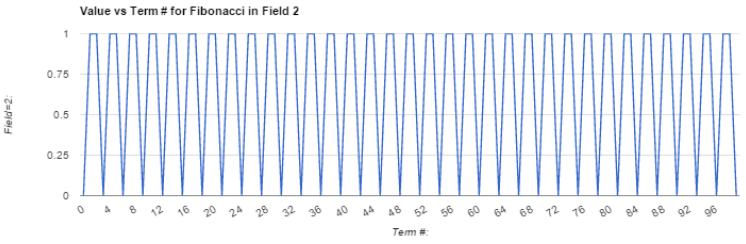
\includegraphics[width=\textwidth]{images/fib_field2.png}
  \caption{Sequence for Fibonacci in $\mathbb{F}_2$ with period 3}
  \label{fig:fib_F2}
\end{figure}
\begin{figure}[H]
  \centering
  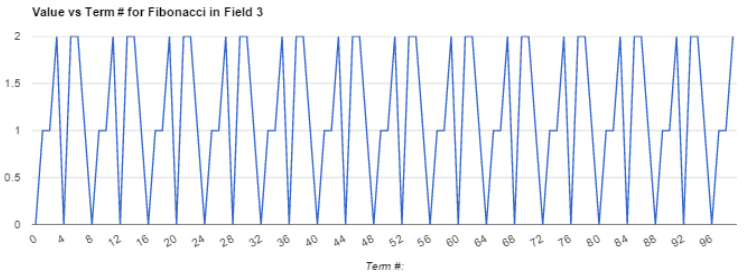
\includegraphics[width=\textwidth]{images/fib_field3.png}
  \caption{Sequence for Fibonacci in $\mathbb{F}_3$ with period 8}
  \label{fig:fib_F3}
\end{figure}
\begin{figure}[!ht]
  \centering
  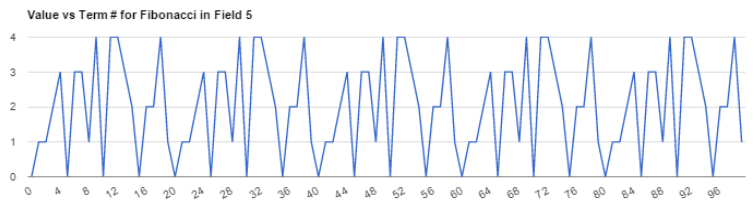
\includegraphics[width=\textwidth]{images/fib_field5.png}
  \caption{Sequence for Fibonacci in $\mathbb{F}_5$ with period 20}
  \label{fig:fib_F5}
\end{figure}
\begin{figure}[!ht]
  \centering
  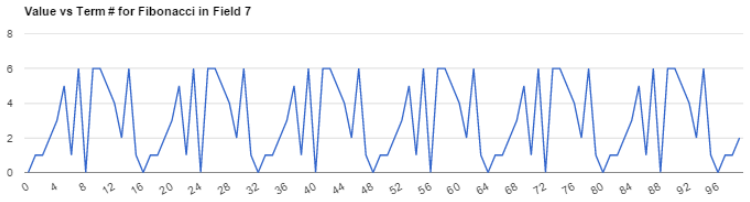
\includegraphics[width=\textwidth]{images/fib_field7.png}
  \caption{Sequence for Fibonacci in $\mathbb{F}_7$ with period 16}
  \label{fig:fib_F7}
\end{figure}

If the reader turns their attention to Figures~\ref{fig:fib_F2} and~\ref{fig:fib_F5}, they'll notice the
pattern that appears every 3 and 20 terms, respectively. These pattern are not a coincidence and are
proven in the next example.
\\

\begin{example}
Looking at $f_n=f_{n-1}+f_{n-2}$ over $\mathbb{F}_2$, we'll see that
$f_{n+3}=f_{n+2}+f_{n+1}=(f_{n+1}+f_{n})+f_{n+1}=f_{n}$.

Recall that $g(n)=2n3^n$ is the closed form solution for the Fibonacci sequence over $\mathbb{F}_5$.
Then computing $g(n+20)$ we get:

\begin{align*}
g(n+20)
&=2(n+20)3^{n+20} \\
&=2(n+20)3^n3^{20} \\
&=2n(3^n)(3^{20})+2(20)(3^n)(3^{20}) \\
&=2n(3^n)(3^{4^{5}})+2(20)(3^n)(3^{4^{5}}) \\
\end{align*}

However, the $ord(3)=4$, so $3^{4^{5}}=1$, and so this simplifies to $2n3^n$. 
\label{ex:period_fib_F5}
\end{example}

The author notes that these were ad-hoc approaches to verifying the period. However, the reader can note
that having a closed-form solution was helpful in verifying a solution. Though we find out in the next
subsection that a closed-form solution cannot always be found.

\subsection{Irreducibility of the Characteristic Polynomial}

The characteristic polynomial for the Fibonacci sequence was able to be factored over $\mathbb{F}_5$.
However, this need not always be the case. A simple explanation is that a problem arises when your roots
to the characteristic equation are not in your field. We see this happens in Example
\ref{ex:cubic-irred}.
\\

\begin{example}
If we're being to asked to solve $h(n)=h(n-3)$ over $\mathbb{F}_5$ where $h(0)=0$, $h(1)=1$, and $h(2)=2$,
then we'll be asked to find the solutions over a 3-dimensional space in $\mathbb{F}_5$ satisfying
$\lambda^{3}-1=(\lambda-1)(\lambda^2+\lambda+1)=0$. But under the $\mathbb{F}_5$, the $h_1(x)=x^2+x+1$ is
irreducible since it has $\deg(h)=2$ and $h(x)\ne 0, \forall x\in \mathbb{F}_5$. 
\label{ex:cubic-irred}
\end{example}

Moreover, it can be calculated that $x^2-x-1$ is irreducible over $\mathbb{F}_2$, $\mathbb{F}_3$,
$\mathbb{F}_7$ as well. To the best of the author's knowledge, little is known between the connection
between the irreducible factors of a characteristic polynomial and the solutions to the basis. Having
knowledge that these polynomials must factor in some field extension seems helpful. However,
interpreting these problems in such a way is outside the scope of this paper.

In conclusion, it's clear that there is much more to learn about defining recursions over a finite
field. Understanding their patterns is important, as well. However, understanding how irreducibility
plays a role in this scenario should be a priority to understanding this problems.

\section{Solving a Conditional Linear Recurrence}

Up until now, the topic has been about finding a closed-form solution for a linear recurrence relation.
However a method exists for solving conditional recurrences -- though it's a little more complex. The
author would like to note that this process is taken directly from~\cite{bib:gen_cond_rec} as it
conveniently explains the process in perfect detail. The reader can note that this process can be
extended to any field as the operations are not necessarily limited to $\mathbb{R}$ or $\mathbb{C}$.

We start by defining a general conditional recurrence relation. Let $\{a_{i,j}\}$ be real numbers for
$0 \le i \le r-1$ and $1 \le j \le s$, and define a sequence ${q_n}$ with given terms $q_i$,
$0 \le i \le s-1$, and for $n \ge s$:

\begin{align*}
q_n=
\begin{cases}
a_{0,1}q_{n-1}+a_{0,2}q_{n-2}+\cdots+a_{0,s}q_{n-s}       & \equiv 0   \mod r \\
a_{1,1}q_{n-1}+a_{1,2}q_{n-2}+\cdots+a_{1,s}q_{n-s}       & \equiv 1   \mod r \\
\vdots                                                                        \\
a_{r-1,1}q_{n-1}+a_{r-1,2}q_{n-2}+\cdots+a_{r-1,s}q_{n-s} & \equiv r-1 \mod r \\
\end{cases}
\end{align*}

We call such a sequence a \textit{general conditional recurrence sequence} with \textit{associated
coefficient matrix}.

\begin{align*}
A=
\begin{bmatrix}
    a_{0,1}   & a_{0,2}   & \cdots  & a_{0,n} \\
    a_{1,1}   & a_{1,2}   & \cdots  & a_{1,n} \\
    \vdots    & \vdots    & \ddots & \vdots  \\
    a_{r-1,1} & a_{r-1,2} & \cdots  & a_{r-1,n}
\end{bmatrix}
\end{align*}

We note that sequence [A068911] is an example of general conditional recurrence sequence where $r=s=2$
and $(a_{0,1},a_{0,2},a_{1,1},a_{1,2})=(2,0,1,1)$. For the sake of this simply understanding the
material, we'll explain the process for when we're given ${a_{i,j}}$ $r \le 3$ and $s \le 3$. Therefore,
we're interested in solving the sequence $q_n$ with initial values $q_0$, $q_1$, $q_2$ for when
$n \ge 3$ by:

\begin{align*}
q_n=
\begin{cases}
a_{0,1}q_{n-1}+a_{0,2}q_{n-2}+a_{0,3}q_{n-3} & \equiv 0 \mod 3 \\
a_{1,1}q_{n-1}+a_{1,2}q_{n-2}+a_{1,3}q_{n-3} & \equiv 1 \mod 3 \\
a_{2,1}q_{n-1}+a_{2,2}q_{n-2}+a_{2,3}q_{n-3} & \equiv 2 \mod 3 \\
\end{cases}
\end{align*}

Our goal is to the sequence as different subsequences that are related by the successor operator, and
then to solve a homogeneous system. To do this, we bring $q_n$ to the other side of the equation, we can
rewrite this as:

\begin{align*}
0=
\begin{cases}
-a_{0,0}q_{n}+a_{0,1}q_{n-1}+a_{0,2}q_{n-2}+a_{0,3}q_{n-3} & \equiv 0 \mod 3 \\
-a_{1,0}q_{n}+a_{1,1}q_{n-1}+a_{1,2}q_{n-2}+a_{1,3}q_{n-3} & \equiv 1 \mod 3 \\
-a_{2,0}q_{n}+a_{2,1}q_{n-1}+a_{2,2}q_{n-2}+a_{2,3}q_{n-3} & \equiv 2 \mod 3 \\
\end{cases}
\end{align*}
We can rewrite these conditional statements by re-indexing their terms. This gives us:
\begin{align*}
-a_{0,0}q_{(n+1)3+0}+a_{0,1}q_{(n+1)3-1}
+a_{0,2}q_{(n+1)3-2}+a_{0,3}q_{(n+1)3-3} = 0 \\
-a_{1,0}q_{(n+1)3+1}+a_{1,1}q_{(n+1)3+0}
+a_{1,2}q_{(n+1)3-1}+a_{1,3}q_{(n+1)3-2} = 0 \\
-a_{2,0}q_{(n+1)3+2}+a_{2,1}q_{(n+1)3+1}
+a_{2,2}q_{(n+1)3-0}+a_{2,3}q_{(n+1)3-1} = 0
\end{align*}

Now, let $Q_n^{(t)}=q_{n}r+t$ for each $0 \le t \le r-1$. We can rewrite the example as:
\begin{align*}
-a_{0,0}Q_{n+1}^{(0)}+a_{0,1}Q_{n}^{(2)}
+a_{0,2}Q_{n}^{(1)}+a_{0,3}Q_{n}^{(0)} = 0 \\
-a_{1,0}Q_{n+1}^{(1)}+a_{1,1}Q_{n+1}^{(0)}
+a_{1,2}Q_{n}^{(2)}+a_{1,3}Q_{n}^{(1)} = 0 \\
-a_{2,0}Q_{n+1}^{(2)}+a_{2,1}Q_{n+1}^{(1)}
+a_{2,2}Q_{n+1}^{(0)}+a_{2,3}Q_{n}^{(2)} = 0
\end{align*}
Therefore, we now have 3 subsequences given by:
\begin{align*}
\left\{Q_n^{(0)}\right\}_{n=0}^{\infty}
=\left\{q_{3n}\right\}_{n=0}^{\infty}   \\
\left\{Q_n^{(1)}\right\}_{n=0}^{\infty}
=\left\{q_{3n+1}\right\}_{n=0}^{\infty} \\
\left\{Q_n^{(2)}\right\}_{n=0}^{\infty}
=\left\{q_{3n+2}\right\}_{n=0}^{\infty}
\end{align*}

which are called the $3$ decimation sequences of $\{q_{n}r+t\}$. At this point, we apply the successor
operator for the sequence $\{Q_n^{(t)}\}_{n=0}^{\infty}$ since $E^{\mu}Q_{n}^{(t)}=Q_{n+\mu}^{(t)}$ for
any $0 \le \mu \le k$, $0 \le t \le r-1$, we rewrite equation as:

\begin{align*}
-a_{0,0}EQ_{n}^{(0)}+a_{0,1}Q_{n}^{(2)}
+a_{0,2}Q_{n}^{(1)}+a_{0,3}Q_{n}^{(0)} = 0 \\
-a_{1,0}EQ_{n}^{(1)}+a_{1,1}EQ_{n}^{(0)}
+a_{1,2}Q_{n}^{(2)}+a_{1,3}Q_{n}^{(1)} = 0 \\
-a_{2,0}EQ_{n}^{(2)}+a_{2,1}EQ_{n}^{(1)}
+a_{2,2}EQ_{n}^{(0)}+a_{2,3}Q_{n}^{(2)} = 0
\end{align*}

However, this can be written as a homogeneous system:

\begin{align*}
\begin{bmatrix}
    a_{0,3}-a_{0,0}E & a_{0,2}          & a_{0,1}          \\
    a_{1,1}E         & a_{1,3}-a_{1,0}E & a_{1,2}          \\
    a_{2,2}          & a_{2,1}E         & a_{2,3}-a_{2,0}E \\
\end{bmatrix}
\begin{bmatrix}
    Q_{n}^{(0)} \\
    Q_{n}^{(1)} \\
    Q_{n}^{(2)}
\end{bmatrix}
=
\begin{bmatrix}
    0 \\
    0 \\
    0
\end{bmatrix}
\end{align*}
This is of the form:
$
[P_{ij}(E)]_{3 \times 3}
\begin{bmatrix}
    Q_{n}^{(0)} \\
    Q_{n}^{(1)} \\
    Q_{n}^{(2)}
\end{bmatrix}
=0
$

At this point, we use a Theorem 2 from~\cite{bib:gen_cond_rec}. We'll declare it below.
\\

\begin{theorem}
If $D=D(E)=detP$, then $\{q_n\}$  satisfies the recurrence relation whose characteristic polynomial is
$D(\lambda^r)$
\label{thm:det-is-char-poly-dxr}
\end{theorem}

Therefore:

\begin{align*}
D
&=detP \\
&=E^3 \\
&- (a_{0,1}a_{1,1}a_{2,1}+a_{0,1}a_{2,2}+a_{0,2}a_{1,1}+a_{1,2}a_{2,1}+a_{0,3}+a_{1,3}+a_{2,3})E^2 \\
&+ (a_{0,3}a_{1,2}a_{2,1}+a_{0,1}a_{1,3}a_{2,2}+a_{0,2}a_{1,1}a_{2,3}+a_{1,3}a_{2,3}+a_{0,3}a_{2,3}+a_{0,3}a_{1,3}-a_{0,2}a_{1,2}a_{2,2})E \\
&-(a_{0,3}a_{1,2}a_{2,1})
\end{align*}

Since $r=3$, by Theorem~\ref{thm:det-is-char-poly-dxr}, we get that when the determinant equals zero,
substituting $\lambda^3$ in for $E$ gives us the characteristic polynomial:

\begin{align*}
\lambda^9
&= (a_{0,1}a_{1,1}a_{2,1}+a_{0,1}a_{2,2}+a_{0,2}a_{1,1}+a_{1,2}a_{2,1}+a_{0,3}+a_{1,3}+a_{2,3})\lambda^6 \\
&- (a_{0,3}a_{1,2}a_{2,1}+a_{0,1}a_{1,3}a_{2,2}+a_{0,2}a_{1,1}a_{2,3}+a_{1,3}a_{2,3}+a_{0,3}a_{2,3}+a_{0,3}a_{1,3}-a_{0,2}a_{1,2}a_{2,2})\lambda^3 \\
&+(a_{0,3}a_{1,2}a_{2,1})
\end{align*}

\subsection{Examples and Observations}

\begin{example}

Suppose $q_n$ is defined like so:
\begin{align*}
q_n=
\begin{cases}
1q_{n-1}+1q_{n-2}+1q_{n-3} & \equiv 0 \mod 3 \\
1q_{n-1}+1q_{n-2}+0q_{n-3} & \equiv 1 \mod 3 \\
2q_{n-1}+1q_{n-2}+0q_{n-3} & \equiv 2 \mod 3 \\
\end{cases}
\end{align*}
Then we follow the previous steps to obtain that:
\begin{align*}
P=
\begin{bmatrix}
    1-E & 1  & 1  \\
    E   & -E & 1  \\
    E   & 2E & -E \\
\end{bmatrix}
\end{align*}
Calculating the determinant, we find that:
\begin{align*}
D=(-E)(E^2-7E+1)
\end{align*}
Substituting $E=\lambda^3$ implies we need to solve $p(\lambda)=\lambda^6-7\lambda^3+1$ -- a degree 6
polynomial whose solutions are our basis for the 6-dimensional vector space that satisfies both
$\{q_n\}$ and ${p_n}$ where $p_n=7p_{n-3}-p_{n-6}$.
\end{example}

The next example showcases the characteristic polynomial can be factored over finite field
$\mathbb{F}_2$ and $\mathbb{F}_4$, but no other tested field. However, a precaution needs to be taken
since the initial conditions need to be altered to satisfy the newly obtained linear recursion. 
\\
\begin{example}
Suppose $q_n$ is defined like so:
\begin{align*}
q_n=
\begin{cases}
2q_{n-1}+0q_{n-2} & \equiv 0 \mod 2 \\
1q_{n-1}+1q_{n-2} & \equiv 1 \mod 2 \\
\end{cases}
\end{align*}
Then, once again, we follow the previous steps to obtain that:
\begin{align*}
P=
\begin{bmatrix}
   -E &    2 \\
    E & -E+1 \\
\end{bmatrix}
\end{align*}
Calculating the determinant, we find that:
\begin{align*}
D=(-E)(-E+1)-(E)(2)=\cdots=E(E-3)
\end{align*}
Substituting $E=\lambda^2$ implies we need to solve $p(\lambda)=\lambda^2-3$ -- a degree 2 polynomial
whose solutions are our basis for the 2-dimensional vector space that satisfies both $\{q_n\}$ and
${p_n}$ where $p_n=3p_{n-2}$. In this case the closed form solution is
$q_n=\left(\frac{2+\sqrt{3}}{3}\right)(\sqrt{3})^n+\frac{2+\sqrt{3}}{3}(-\sqrt{3})^n$. However, for this
to hold, the $q_0$ must be set to $q_0=\frac{4}{3}$ since $q_2={4}=3q_0$. 

Similarly, the reader can note that if factoring $\lambda^2-3$ over $\mathbb{F}_2$ and $\mathbb{F}_4$ is
possible. Similarly, since the the sequence outputs all zeros, and so the initial conditions needed to
be modified as well. 

It's output can be seen in the table below.

\begin{table}[ht]
\centering
\begin{tabular}{lllllllllllllllll}
\toprule
Term \#:  & 0 & 1 & 2 & 3 & 4  & 5  & 6  & 7  & 8   & 9   & 10  & 11  & 12  & 13   & 14   & 15                \\
\midrule
Field=$\mathbb{R}$:  & 1 & 2 & 4 & 6 & 12 & 18 & 36 & 54 & 108 & 162 & 324 & 486 & 972 & 1458 & 2916 & 4374   \\
Field=$\mathbb{F}_2$:  & 1 & 0 & 0 & 0 & 0  & 0  & 0  & 0  & 0   & 0   & 0   & 0   & 0   & 0    & 0    & 0    \\
Field=$\mathbb{F}_3$:  & 1 & 2 & 1 & 0 & 0  & 0  & 0  & 0  & 0   & 0   & 0   & 0   & 0   & 0    & 0    & 0    \\
Field=$\mathbb{F}_4$:  & 1 & 0 & 0 & 0 & 0  & 0  & 0  & 0  & 0   & 0   & 0   & 0   & 0   & 0    & 0    & 0    \\
Field=$\mathbb{F}_5$:  & 1 & 2 & 4 & 1 & 2  & 3  & 1  & 4  & 3   & 2   & 4   & 1   & 2   & 3    & 1    & 4    \\
Field=$\mathbb{F}_7$:  & 1 & 2 & 4 & 6 & 5  & 4  & 1  & 5  & 3   & 1   & 2   & 3   & 6   & 2    & 4    & 6    \\
Field=$\mathbb{F}_8$:  & 1 & 0 & 0 & 0 & 0  & 0  & 0  & 0  & 0   & 0   & 0   & 0   & 0   & 0    & 0    & 0    \\
Field=$\mathbb{F}_9$:  & 1 & 2 & 1 & 0 & 0  & 0  & 0  & 0  & 0   & 0   & 0   & 0   & 0   & 0    & 0    & 0    \\
Field=$\mathbb{F}_{11}$: & 1 & 2 & 4 & 6 & 1  & 7  & 3  & 10 & 9   & 8   & 5   & 2   & 4   & 6    & 1    & 7  \\
Field=$\mathbb{F}_{13}$: & 1 & 2 & 4 & 6 & 12 & 5  & 10 & 2  & 4   & 6   & 12  & 5   & 10  & 2    & 4    & 6  \\
\bottomrule
\end{tabular}
\caption{Output of $q_n$ of type (2,0,1,1) over various fields}
\label{my-label}
\end{table}

However, over other tested fields, no closed form solution can be found since $\lambda^2-3$ is irreducible. 
\end{example}

\section{Conclusion}

Therefore, it can be concluded that there there are many applications of finite fields to the study of linear
recurrences. From the study of periods to the more important study of irreducibles in characteristic
polynomials, for conditional or unconditional recurrences, these will play a role in understanding recurrences
altogether. 

\begin{thebibliography}{9}

\bibitem{bib:solve-lin-rec-field}
  K. Conrad,
  \emph{Solving Linear Recursion over all Fields},
  Expository Paper, \textit{http://www.math.uconn.edu/~kconrad/blurbs/linmultialg/linearrecursion.pdf}

\bibitem{bib:successor-explained}
  D. Detemple, W. Webb,
  \emph{Combinatorial Reasoning},
  (Chapter 5.2.1 - 5.2.2), 
  2014. Online at \texttt{https://goo.gl/E7VT7m} %used a URL shortener to eliminate a bug
  
\bibitem{bib:gen_cond_rec}
  D. Panario, M. Sahin, Q. Wang, W. Webb,
  \emph{General conditional recurrences},
  Applied Mathematics and Computation 243
  (2014) 220-231.

\bibitem{bib:lfsr}
  The University of Sydney
  \emph{Linear Feedback Shift Registers}
  Math3024 Elementary Cryptography and Protocols
  Online at \texttt{http://goo.gl/RMFLh3}

\end{thebibliography}

\end{document}
